%----------------------------------------------------------------------------------------
%	CHAPTER - INTRODUCTUION
%----------------------------------------------------------------------------------------

\chapter{Introduction} % Main chapter title

\label{ChapterIntroduction} % Change X to a consecutive number; for referencing this chapter elsewhere, use \ref{ChapterX}

%----------------------------------------------------------------------------------------
%	SECTION 1
%----------------------------------------------------------------------------------------

\section{Introduction}

Within the next five to ten years, virtual reality is predicted to achieve mainstream adoption and entering the so called "Plateau of Productivity" \citep{Gartner2015}.

Virtual reality gets increasing awareness in the news and according to \cite{Gartner2015} will already even achieve mainstream adoption within the next five to ten years.

With the release of the Occulus Rift in 2015, the HTC Vive in 2016 and the awaited Sony XYZ, virtual reality is ... the news. Although we only see the first version of consumer products, \cite{Gartner2015} predicts that within the next five to ten years, virtual reality will achieve mainstream adoption and enters the so called "Plateau of Producitivity".

blub
\cite{Safrudin2015}
blub


According to Gartner, people generally get over-excited about new technologies in the early days followed by a period of disappointment (after it fails to deliver to the heightened expectations). Beyond that phase some solutions mature and deliver on the initial promise, rebuilding hype/excitement and acceptance of the technology.


 The report is from Gartner, a technology research firm. The group puts out an annual report on emerging tech called the Gartner Hype Cycle, and this year's report puts VR on the upswing toward mainstream adoption. Tech Insider was given access to the full report.
 See virtual reality below, sliding up the "Slope of Enlightenment" between "Autonomous Field Vehicles" and "Gesture Control?" Don't let the analyst firm's term for where VR is at on the Hype Cycle throw you off — it's just Gartner's way of measuring where emerging technologies are in the zeitgeist.
 In plain English, that means VR is close to the point where it's widely understood by the general public. But that doesn't necessarily make it a mainstream technology. 

Gartner believes that both AR and VR will still take 5 to 10 years to reach the “Plateau of Productivity” (mainstream adoption). Perhaps this may be true for widespread adoption in the enterprise market. However, I think we’ll be seeing adoption in the consumer market much sooner. VR headsets are readily available (with more to be released soon). With AR we don’t have commercially available AR headsets in the market yet. We have AR smartphone solutions and some people managed to get their hands on a Google Glass headset when the programme was still running.



The common phrase “It’s a small world” becomes true everyday – with people and things getting more and more connected by the Internet and becoming more mobile. Furthermore, with advances in technology, information reaches faster and smarter to you. We become more productive in our daily work assisted by technology so small enough that it fits in our pockets and we are able to carry it along whole day. These devices are mostly represented by smartphones – which have become so essential for our life – that we haven even forgotten how life could look like without them.





\begin{figure}[h]
	\begin{center}
		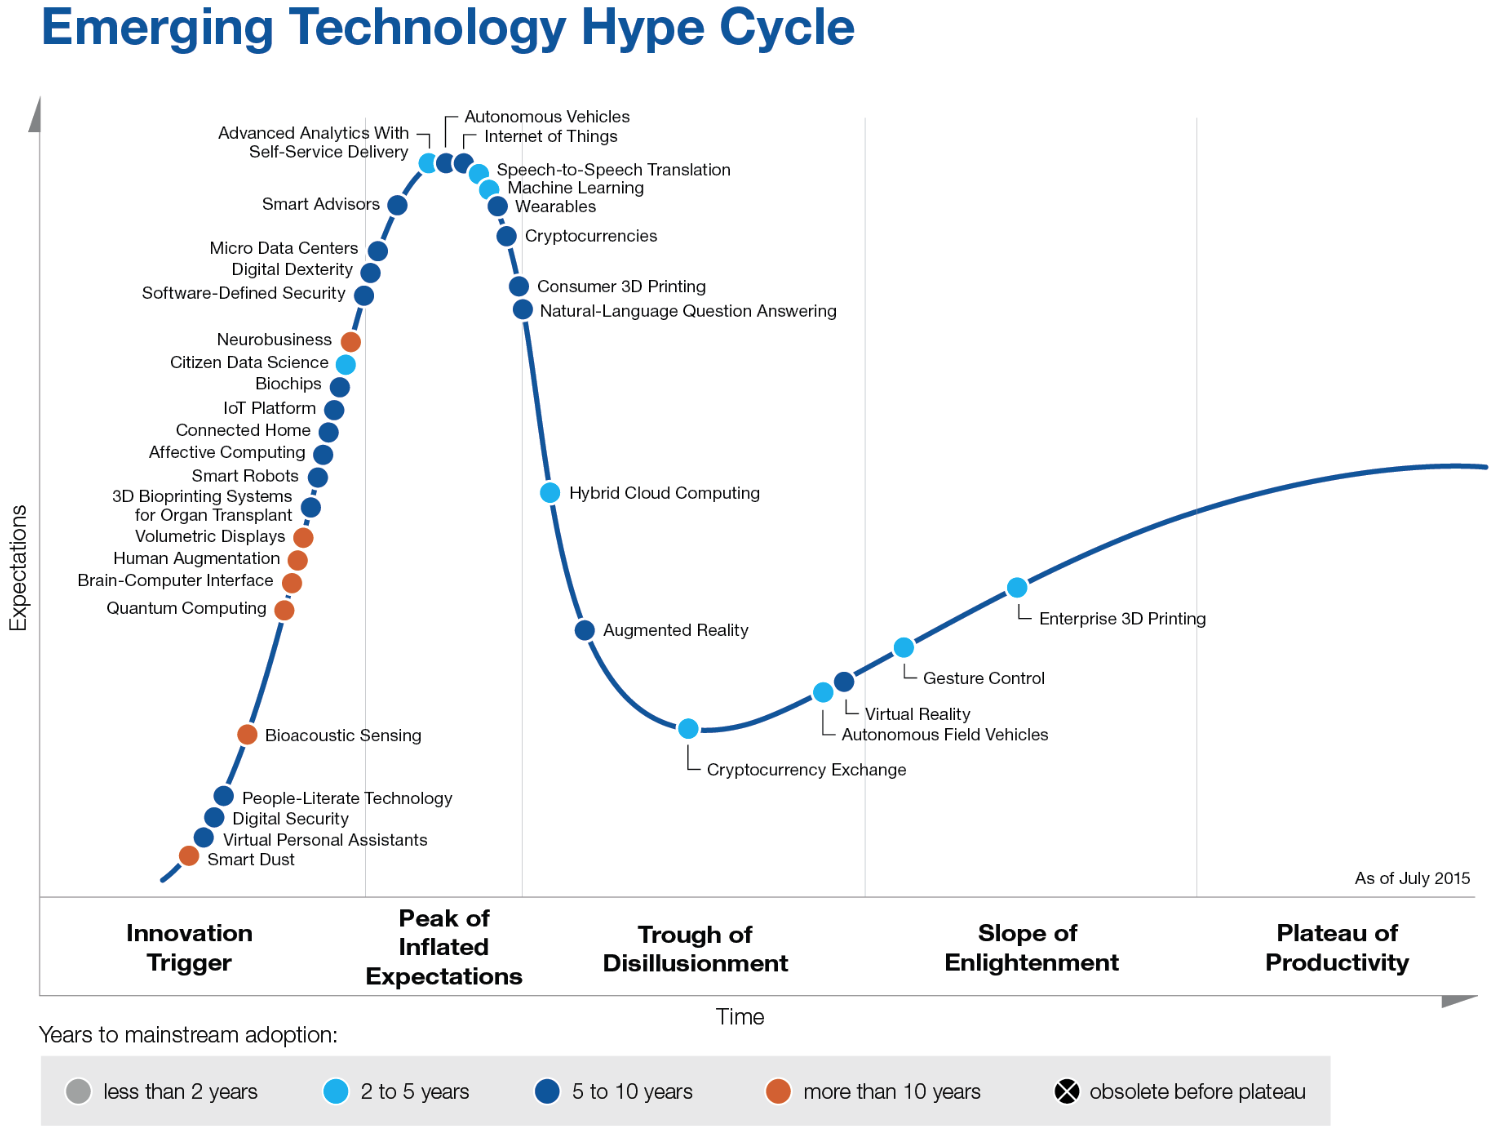
\includegraphics[width=11cm]{03_Figures/03_Gartner/Gartner_EmergingTech2015.png}
		\caption[Emerging Technology Hype Cycle]{Emerging Technology Hype Cycle \citep{Gartner2015b}}
		\label{fig:dsrcycle}
	\end{center}
\end{figure}


The focus of this thesis is on the possibilitios of enhanced user interaction with data in virtual reality by utilizing the additional sensor information of gesture controllers and 360° motion tracking.

In the following subchapters, more background information about the topic is given as well as the definition of the problem statement. Based on this, the thesis statement is proposed and research questions are derived from. Following this, the delineations and limitations are presented before this chapter is closed with the structure of the thesis and a brief overview of the chapters and their corelations.


%----------------------------------------------------------------------------------------
%	SECTION 2
%----------------------------------------------------------------------------------------

\section{Background}

blub


%----------------------------------------------------------------------------------------
%	SECTION 3
%----------------------------------------------------------------------------------------

\section{Problem Statement}

blub


%----------------------------------------------------------------------------------------
%	SECTION 4
%----------------------------------------------------------------------------------------

\section{Thesis Statement}
... therefore the tesis statement is as follows: \newline
\textit{The interaction with multidimensional data in virtual reality can be enhanced by utilizing gesture controllers and 360° motion tracking and using the derived sensor information.}

%----------------------------------------------------------------------------------------
%	SECTION 5
%----------------------------------------------------------------------------------------

\section{Research question}

\textit{SRQ 1: Which ways of interaction with multi-dimensional exist and what are their strengths and weaknesses?}
\newline
\textit{SRQ 2: How can retrieved sensor information be used to enhance the interaction model with multidimensional data?}



%----------------------------------------------------------------------------------------
%	SECTION 6
%----------------------------------------------------------------------------------------

\section{Research Objectives}

blub


%----------------------------------------------------------------------------------------
%	SECTION 7
%----------------------------------------------------------------------------------------

% \section{Short Overview}


%----------------------------------------------------------------------------------------
%	SECTION 8
%----------------------------------------------------------------------------------------

\section{Delineations and Limitations}

blub


%----------------------------------------------------------------------------------------
%	SECTION 9
%----------------------------------------------------------------------------------------

% \section{Underlying Assumptions}


%----------------------------------------------------------------------------------------
%	SECTION 10
%----------------------------------------------------------------------------------------

% \section{Definition of terms and concepts}


%----------------------------------------------------------------------------------------
%	SECTION 11
%----------------------------------------------------------------------------------------

% \section{Significance}


%-----------------------------------
%	SUBSECTION 1
%-----------------------------------

% \subsection{Theoretical}


%-----------------------------------
%	SUBSECTION 2
%-----------------------------------

% \subsection{Practical}


%----------------------------------------------------------------------------------------
%	SECTION 12
%----------------------------------------------------------------------------------------

\section{Thesis structure and brief chapter overviews}

blub


%----------------------------------------------------------------------------------------
%	SECTION 13
%----------------------------------------------------------------------------------------

% \section{Any other institutional requirement not covered here}



